% file: pacific_atlantic_water_flow.tex

\problemsection{Pacific Atlantic Water Flow}
\label{problem:pacific_atlantic_water_flow}
\marginnote{This problem leverages depth-first search (DFS) or breadth-first search (BFS) to determine cells from which water can flow to both the Pacific and Atlantic oceans.}
    
The \textbf{Pacific Atlantic Water Flow} problem is a graph theory challenge that involves identifying matrix coordinates from which water can flow to both the Pacific and Atlantic oceans under specific conditions.

\section*{Problem Statement}
Imagine a continent as an \(m \times n\) matrix of non-negative integers where each cell represents the height of a unit of terrain. The Pacific Ocean borders the continent to the west (left edge) and north (top edge), while the Atlantic Ocean borders it to the east (right edge) and south (bottom edge). Water flows from a cell to any adjacent cell with equal or lower elevation.

The task is to identify all the cells from where water can reach both the Pacific and Atlantic oceans. These cells are at crossroads where water, if allowed to flow naturally according to the rules, would be able to reach both oceans.

\section*{Examples}

\textit{Example 1:}

\begin{verbatim}
Input:
matrix = [
  [1, 2, 2, 3, 5],
  [3, 2, 3, 4, 4],
  [2, 4, 5, 3, 1],
  [6, 7, 1, 4, 5],
  [5, 1, 1, 2, 4]
]
Output:
[[0,4],[1,3],[1,4],[2,2],[3,0],[3,1],[4,0]]
\end{verbatim}

\textit{Example 2:}

\begin{verbatim}
Input:
matrix = [
  [2, 1],
  [1, 2]
]
Output:
[[0,0],[0,1],[1,0],[1,1]]
\end{verbatim}

LeetCode link: \href{https://leetcode.com/problems/pacific-atlantic-water-flow/}{Pacific Atlantic Water Flow}\index{LeetCode}

\marginnote{\href{https://leetcode.com/problems/pacific-atlantic-water-flow/}{[LeetCode Link]}\index{LeetCode}}
\marginnote{\href{https://www.geeksforgeeks.org/pacific-atlantic-water-flow/}{[GeeksForGeeks Link]}\index{GeeksForGeeks}}
\marginnote{\href{https://www.hackerrank.com/challenges/pacific-atlantic-water-flow/problem}{[HackerRank Link]}\index{HackerRank}}
\marginnote{\href{https://app.codesignal.com/challenges/pacific-atlantic-water-flow}{[CodeSignal Link]}\index{CodeSignal}}
\marginnote{\href{https://www.interviewbit.com/problems/pacific-atlantic-water-flow/}{[InterviewBit Link]}\index{InterviewBit}}
\marginnote{\href{https://www.educative.io/courses/grokking-the-coding-interview/RM8y8Y3nLdY}{[Educative Link]}\index{Educative}}
\marginnote{\href{https://www.codewars.com/kata/pacific-atlantic-water-flow/train/python}{[Codewars Link]}\index{Codewars}}

\section*{Algorithmic Approach}

\subsection*{Main Concept}
To solve this problem, we can perform a search from the oceans inwards using either Depth-First Search (DFS) or Breadth-First Search (BFS), marking the cells that can be reached by water flowing from each ocean. Finally, we identify the intersection of the cells reachable from both oceans.

\begin{enumerate}
    \item \textbf{Initialize Reachability Sets:}
    \begin{itemize}
        \item Create two sets, \texttt{pacific} and \texttt{atlantic}, to keep track of cells reachable by water flowing to the Pacific and Atlantic oceans, respectively.
    \end{itemize}
    
    \item \textbf{Perform DFS/BFS for Both Oceans:}
    \begin{itemize}
        \item Iterate through each row and perform DFS/BFS starting from the leftmost (Pacific) and rightmost (Atlantic) cells.
        \item Iterate through each column and perform DFS/BFS starting from the topmost (Pacific) and bottommost (Atlantic) cells.
    \end{itemize}
    
    \item \textbf{Identify Common Reachable Cells:}
    \begin{itemize}
        \item The cells present in both \texttt{pacific} and \texttt{atlantic} sets are the desired cells where water can flow to both oceans.
    \end{itemize}
\end{enumerate}

This approach ensures that each cell is visited at most twice (once for each ocean), leading to an efficient solution.

\marginnote{DFS and BFS efficiently explore all possible paths from the ocean boundaries, ensuring all reachable cells are accounted for without redundant processing.}

\section*{Complexities}

\begin{itemize}
	\item \textbf{Time Complexity:} Let \(m\) be the number of rows and \(n\) be the number of columns in the matrix. The time complexity is \(O(m \cdot n)\) for both DFS and BFS approaches, as each cell is processed once for each ocean.
	
	\item \textbf{Space Complexity:} The space complexity is \(O(m \cdot n)\) due to the storage of two separate matrices (or equivalent data structures) to keep track of reachable cells from both oceans.
\end{itemize}

\newpage % Start Python Implementation on a new page
\section*{Python Implementation}

\marginnote{Implementing DFS or BFS requires careful handling of grid boundaries and visited cells to ensure accurate and efficient traversal.}

Below is the complete Python code for the water flow problem using Depth-First Search (DFS):

\begin{fullwidth}
\begin{lstlisting}[language=Python]
class Solution(object):
    def pacificAtlantic(self, matrix):
        if not matrix or not matrix[0]: return []
        
        def dfs(x, y, visited, prevHeight):
            if (x, y) in visited or \
               x < 0 or x >= len(matrix) or y < 0 or y >= len(matrix[0]) or \
               matrix[x][y] < prevHeight:
                return
            visited.add((x, y))
            for dx, dy in [(1, 0), (-1, 0), (0, 1), (0, -1)]:
                dfs(x + dx, y + dy, visited, matrix[x][y])

        pacific = set()
        atlantic = set()

        for i in range(len(matrix)):
            dfs(i, 0, pacific, matrix[i][0])
            dfs(i, len(matrix[0]) - 1, atlantic, matrix[i][-1])
        for j in range(len(matrix[0])):
            dfs(0, j, pacific, matrix[0][j])
            dfs(len(matrix) - 1, j, atlantic, matrix[-1][j])

        return list(pacific & atlantic)
        
# You can call the function with any matrix input to test.
# For example:
# solution = Solution()
# matrix = [
#     [1, 2, 2, 3, 5],
#     [3, 2, 3, 4, 4],
#     [2, 4, 5, 3, 1],
#     [6, 7, 1, 4, 5],
#     [5, 1, 1, 2, 4]
# ]
# print(solution.pacificAtlantic(matrix))  # Output: [[0,4],[1,3],[1,4],[2,2],[3,0],[3,1],[4,0]]
\end{lstlisting}
\end{fullwidth}

\begin{fullwidth}
\begin{lstlisting}[language=Python]
class Solution(object):
    def pacificAtlantic(self, matrix):
        if not matrix or not matrix[0]: return []
        
        def dfs(x, y, visited, prevHeight):
            if (x, y) in visited or \
               x < 0 or x >= len(matrix) or y < 0 or y >= len(matrix[0]) or \
               matrix[x][y] < prevHeight:
                return
            visited.add((x, y))
            for dx, dy in [(1, 0), (-1, 0), (0, 1), (0, -1)]:
                dfs(x + dx, y + dy, visited, matrix[x][y])

        pacific = set()
        atlantic = set()

        for i in range(len(matrix)):
            dfs(i, 0, pacific, matrix[i][0])
            dfs(i, len(matrix[0]) - 1, atlantic, matrix[i][-1])
        for j in range(len(matrix[0])):
            dfs(0, j, pacific, matrix[0][j])
            dfs(len(matrix) - 1, j, atlantic, matrix[-1][j])

        return list(pacific & atlantic)
\end{lstlisting}
\end{fullwidth}

This implementation uses Depth-First Search (DFS) from the edge cells adjacent to each ocean and marks cells that can be reached by water flowing from each ocean. By finding the intersection of cells reachable by both oceans, we obtain the desired cells where water can flow to both the Pacific and Atlantic oceans.

\section*{Explanation}

The provided Python implementation defines a class \texttt{Solution} which contains the method \texttt{pacificAtlantic}. Here's a detailed breakdown of the implementation:

\begin{itemize}
    \item \textbf{Edge Case Handling:}
    \begin{itemize}
        \item If the input \texttt{matrix} is empty or contains no columns, the function returns an empty list, as there are no cells to process.
    \end{itemize}
    
    \item \textbf{Depth-First Search (DFS) Function:}
    \begin{itemize}
        \item The nested \texttt{dfs} function takes the current cell coordinates \texttt{x} and \texttt{y}, a \texttt{visited} set to track reachable cells, and \texttt{prevHeight} to ensure water can flow from higher or equal elevation to lower elevation.
        \item It checks for the following conditions:
        \begin{itemize}
            \item If the current cell \((x, y)\) has already been visited.
            \item If the current cell is out of the matrix boundaries.
            \item If the current cell's height is less than the previous cell's height, preventing water from flowing uphill.
        \end{itemize}
        \item If none of the above conditions are met, the cell is marked as visited.
        \item The function then recursively calls itself for all four adjacent cells (up, down, left, right).
    \end{itemize}
    
    \item \textbf{Initializing Reachability Sets:}
    \begin{itemize}
        \item Two sets, \texttt{pacific} and \texttt{atlantic}, are initialized to keep track of cells reachable by water flowing to the Pacific and Atlantic oceans, respectively.
    \end{itemize}
    
    \item \textbf{Performing DFS from Ocean Boundaries:}
    \begin{itemize}
        \item Iterate through each row:
        \begin{itemize}
            \item Perform DFS starting from the first column (Pacific Ocean).
            \item Perform DFS starting from the last column (Atlantic Ocean).
        \end{itemize}
        \item Iterate through each column:
        \begin{itemize}
            \item Perform DFS starting from the first row (Pacific Ocean).
            \item Perform DFS starting from the last row (Atlantic Ocean).
        \end{itemize}
    \end{itemize}
    
    \item \textbf{Identifying Common Reachable Cells:}
    \begin{itemize}
        \item The intersection of \texttt{pacific} and \texttt{atlantic} sets (\texttt{pacific \& atlantic}) contains the cells from which water can flow to both oceans.
        \item Convert the intersection set to a list and return it as the result.
    \end{itemize}
\end{itemize}

This approach ensures that each cell is visited at most twice (once for each ocean), leading to an efficient and optimized solution.

\section*{Why This Approach}

The Depth-First Search (DFS) approach is chosen for its effectiveness in exploring all possible paths from the ocean boundaries inward. By starting DFS from the cells adjacent to each ocean, we can systematically mark all cells that are reachable by water flowing from that ocean. The intersection of these reachable cells from both oceans provides the desired solution. This method efficiently handles the constraints of water flow direction and elevation, ensuring that each relevant cell is accurately accounted for without redundant processing.

\section*{Alternative Approaches}

An alternative approach involves using Breadth-First Search (BFS) instead of DFS. BFS can be implemented using a queue and may be more intuitive for some, as it explores cells level by level. Both DFS and BFS have similar time and space complexities for this problem, but BFS might offer better performance on graphs with a larger breadth. Additionally, one could optimize space by using a single visited matrix with different markers for each ocean, but maintaining separate sets or matrices tends to be clearer and less error-prone.

Another possibility is to use dynamic programming to compute reachable cells, but this is generally more complex and less straightforward compared to the DFS/BFS approaches.

\section*{Similar Problems to This One}

Similar problems that involve traversal or pathfinding in a grid or matrix environment include:
    
\begin{itemize}
    \item \textbf{Number of Islands:} Counting distinct islands in a grid.
    \index{Number of Islands}
    
    \item \textbf{Walls and Gates:} Filling each empty room with the distance to its nearest gate.
    \index{Walls and Gates}
    
    \item \textbf{Longest Increasing Path in a Matrix:} Finding the longest path in a matrix where each step must go to a strictly higher value.
    \index{Longest Increasing Path in a Matrix}
    
    \item \textbf{Surrounded Regions:} Capturing all regions surrounded by 'X's by flipping surrounded 'O's to 'X's.
    \index{Surrounded Regions}
    
    \item \textbf{Max Area of Island:} Finding the largest island's area in a grid.
    \index{Max Area of Island}
\end{itemize}

\section*{Things to Keep in Mind and Tricks}

\begin{itemize}
    \item \textbf{Understanding Flow Directions:} Water can only flow from higher or equal elevation to lower elevation. Ensure that the traversal respects this constraint to avoid incorrect reachability.
    \index{Flow Directions}
    
    \item \textbf{Handling Edge Cells:} Cells on the borders of the matrix are adjacent to the oceans. Starting DFS/BFS from these cells ensures that all reachable cells are appropriately marked.
    \index{Edge Cells}
    
    \item \textbf{Avoiding Redundant Traversals:} Utilize visited sets or matrices to keep track of already processed cells, preventing unnecessary computations and infinite loops.
    \index{Avoiding Redundancy}
    
    \item \textbf{Efficient Data Structures:} Using sets for visited cells allows for \(O(1)\) lookup times, enhancing the overall efficiency of the algorithm.
    \index{Efficient Data Structures}
    
    \item \textbf{Optimizing Traversal Order:} While the order of traversing neighbors (up, down, left, right) doesn't affect the final result, maintaining a consistent order can aid in debugging and understanding the traversal process.
    \index{Traversal Order}
    
    \item \textbf{Intersection of Sets:} After marking reachable cells from both oceans, computing the intersection efficiently identifies the cells that satisfy both conditions.
    \index{Set Intersection}
\end{itemize}

\section*{Corner and Special Cases}

To ensure robustness and correctness, consider testing the following corner cases:

\begin{itemize}
    \item \textbf{Empty Matrix:} An empty matrix should return an empty list as there are no cells to process.
    \index{Corner Cases}
    
    \item \textbf{Single Cell:} A matrix with only one cell, which can either be land or water. Verify that the function handles this minimal case correctly.
    \index{Corner Cases}
    
    \item \textbf{All Cells Can Reach Both Oceans:} A matrix where all cells have high enough elevation to allow water to flow to both oceans.
    \index{Corner Cases}
    
    \item \textbf{No Cells Can Reach Both Oceans:} A matrix where no cell allows water to flow to both oceans simultaneously.
    \index{Corner Cases}
    
    \item \textbf{Cells Only Reach One Ocean:} A matrix where some cells can reach only the Pacific or only the Atlantic Ocean.
    \index{Corner Cases}
    
    \item \textbf{High Elevation Barriers:} Matrices with high elevation barriers that block water flow between certain regions, affecting reachability.
    \index{Corner Cases}
    
    \item \textbf{Large Matrix:} Very large matrices to test the performance and ensure that the algorithm scales efficiently without excessive memory usage or stack overflow (in the case of recursive DFS).
    \index{Corner Cases}
    
    \item \textbf{Matrix with Uniform Elevation:} A matrix where all cells have the same elevation, allowing unrestricted water flow.
    \index{Corner Cases}
    
    \item \textbf{Multiple Water Flow Paths:} Matrices that have multiple distinct paths for water to flow to both oceans.
    \index{Corner Cases}
    
    \item \textbf{Non-Rectangular Matrices:} Although the problem typically assumes a rectangular matrix, testing with non-uniform row lengths (if allowed) can ensure that the function handles such cases gracefully.
    \index{Corner Cases}
\end{itemize}

\section*{Visual Representation}
\begin{figure}[h]
    \centering
    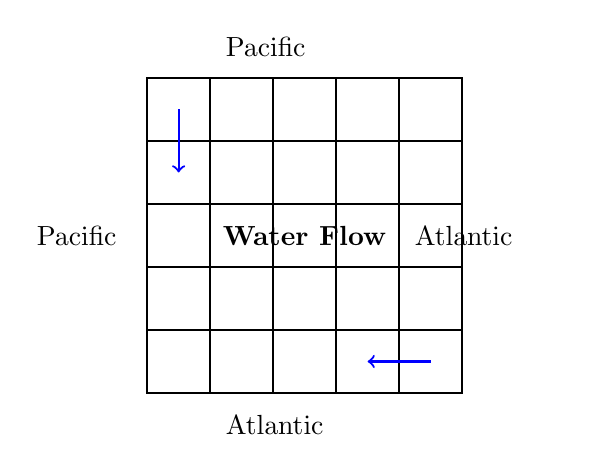
\begin{tikzpicture}[scale=0.8]
        % Grid representation
        \foreach \x in {0,...,4}
            \foreach \y in {0,...,4}
                \draw[thick] (\x,\y) rectangle +(1,1);
        
        % Ocean labels
        \node[text width=2cm] at (-0.5,2.5) {Pacific};
        \node[text width=2cm] at (5.5,2.5) {Atlantic};
        \node[text width=2cm] at (2.5,5.5) {Pacific};
        \node[text width=2cm] at (2.5,-0.5) {Atlantic};
        
        % Flow arrows
        \draw[->,thick,blue] (0.5,4.5) -- (0.5,3.5);
        \draw[->,thick,blue] (4.5,0.5) -- (3.5,0.5);
        
        \node at (2.5,2.5) {\textbf{Water Flow}};
    \end{tikzpicture}
    \caption{Water Flow Directions in the Grid}
    \label{fig:water_flow}
\end{figure}

\section*{Performance Optimization Techniques}
\begin{description}
    \item[Memory Usage] 
    \begin{itemize}
        \item Use bit manipulation for visited states
        \item Reuse existing matrix for marking
        \item Optimize set operations
    \end{itemize}
    
    \item[Time Efficiency]
    \begin{itemize}
        \item Early termination conditions
        \item Direction-based pruning
        \item Cached intermediate results
    \end{itemize}
\end{description}

\printindex